\usetikzlibrary{shapes.geometric}
\usetikzlibrary{arrows.meta}
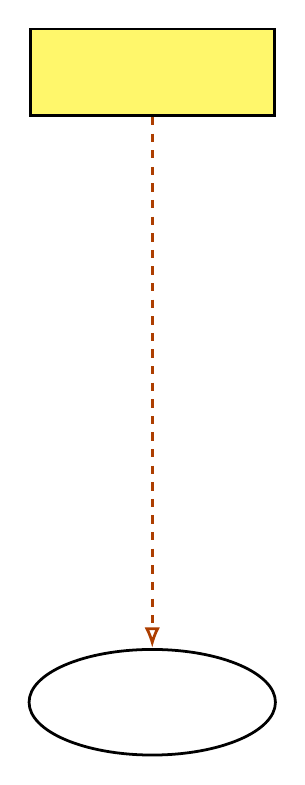
\begin{tikzpicture}

    
    \node[draw={rgb,255:red,0;green,0;blue,0}, fill={rgb,255:red,255;green,255;blue,255}, text={rgb,255:red,0;green,0;blue,0}, line width=1pt, ellipse, minimum width=3.129cm, minimum height=1.341cm] (ndNode2) at (8,1.5) {};
    
    \node[draw={rgb,255:red,0;green,0;blue,0}, fill={rgb,255:red,255;green,247;blue,107}, text={rgb,255:red,0;green,0;blue,0}, line width=1pt, rectangle, minimum width=3.097cm, minimum height=1.099cm] (ndNode3) at (8,9.5) {};
    \draw[draw={rgb,255:red,173;green,62;blue,0}, line width=1pt, dashed, -{Latex[open]}] (ndNode3) -- (ndNode2);
\end{tikzpicture}
